\chapter{Testing and Experimentation} 
This section provides information on the software and hardware tests of the NPSC. It starts by providing an overview of the model used to test the NPSC. It continues by providing all unit tests and system tests performed not the NPSC. Lastly, it explains the current, temperature and light experiments done on the Ring.


%%%%%%%%%%%%%%%%%%%%%%%%%%%%%%%%%%%%%%%%%%%%%%%%%%%%%%%%%%%%%%%%%%%%%%%%%%%%%%%%%%%%
% SECTION: Overview
%%%%%%%%%%%%%%%%%%%%%%%%%%%%%%%%%%%%%%%%%%%%%%%%%%%%%%%%%%%%%%%%%%%%%%%%%%%%%%%%%%%%
\section{Overview}
Debugging an embedded system is one of the worst things in life, especially when there are logical errors in the program. In an embedded system like the NPSC which is made out of modules interacting with each other at different levels of the hierarchy, finding an error would be a difficult task as the error would have to be tracked down to the modules at lower levels. To reduce debugging time, it is essential that each module is independently and thoroughly tested. To achieve this, the verification steps of the v-diagram of the NPSC shown in \cref{fig:v_diagram} are implemented.\\
The hardware modules and framework are tested by analyzing the data transmitted between the STM and these hardware modules, and by running a set of unit tests on the framework code. The sub-systems of the NPSC are tested by running a set of software tests. Following the integration tests is the system test which consists of using the device to ensure that the system requirements have been met. The last verification steps consist of verifying that the device is an alarm-clock able to produce light of wavelength around 460nm and able to fit in a $25*25*10 cm^3$ case. 
\begin{landscape} 
	\begin{figure}[ht]
		\centering
		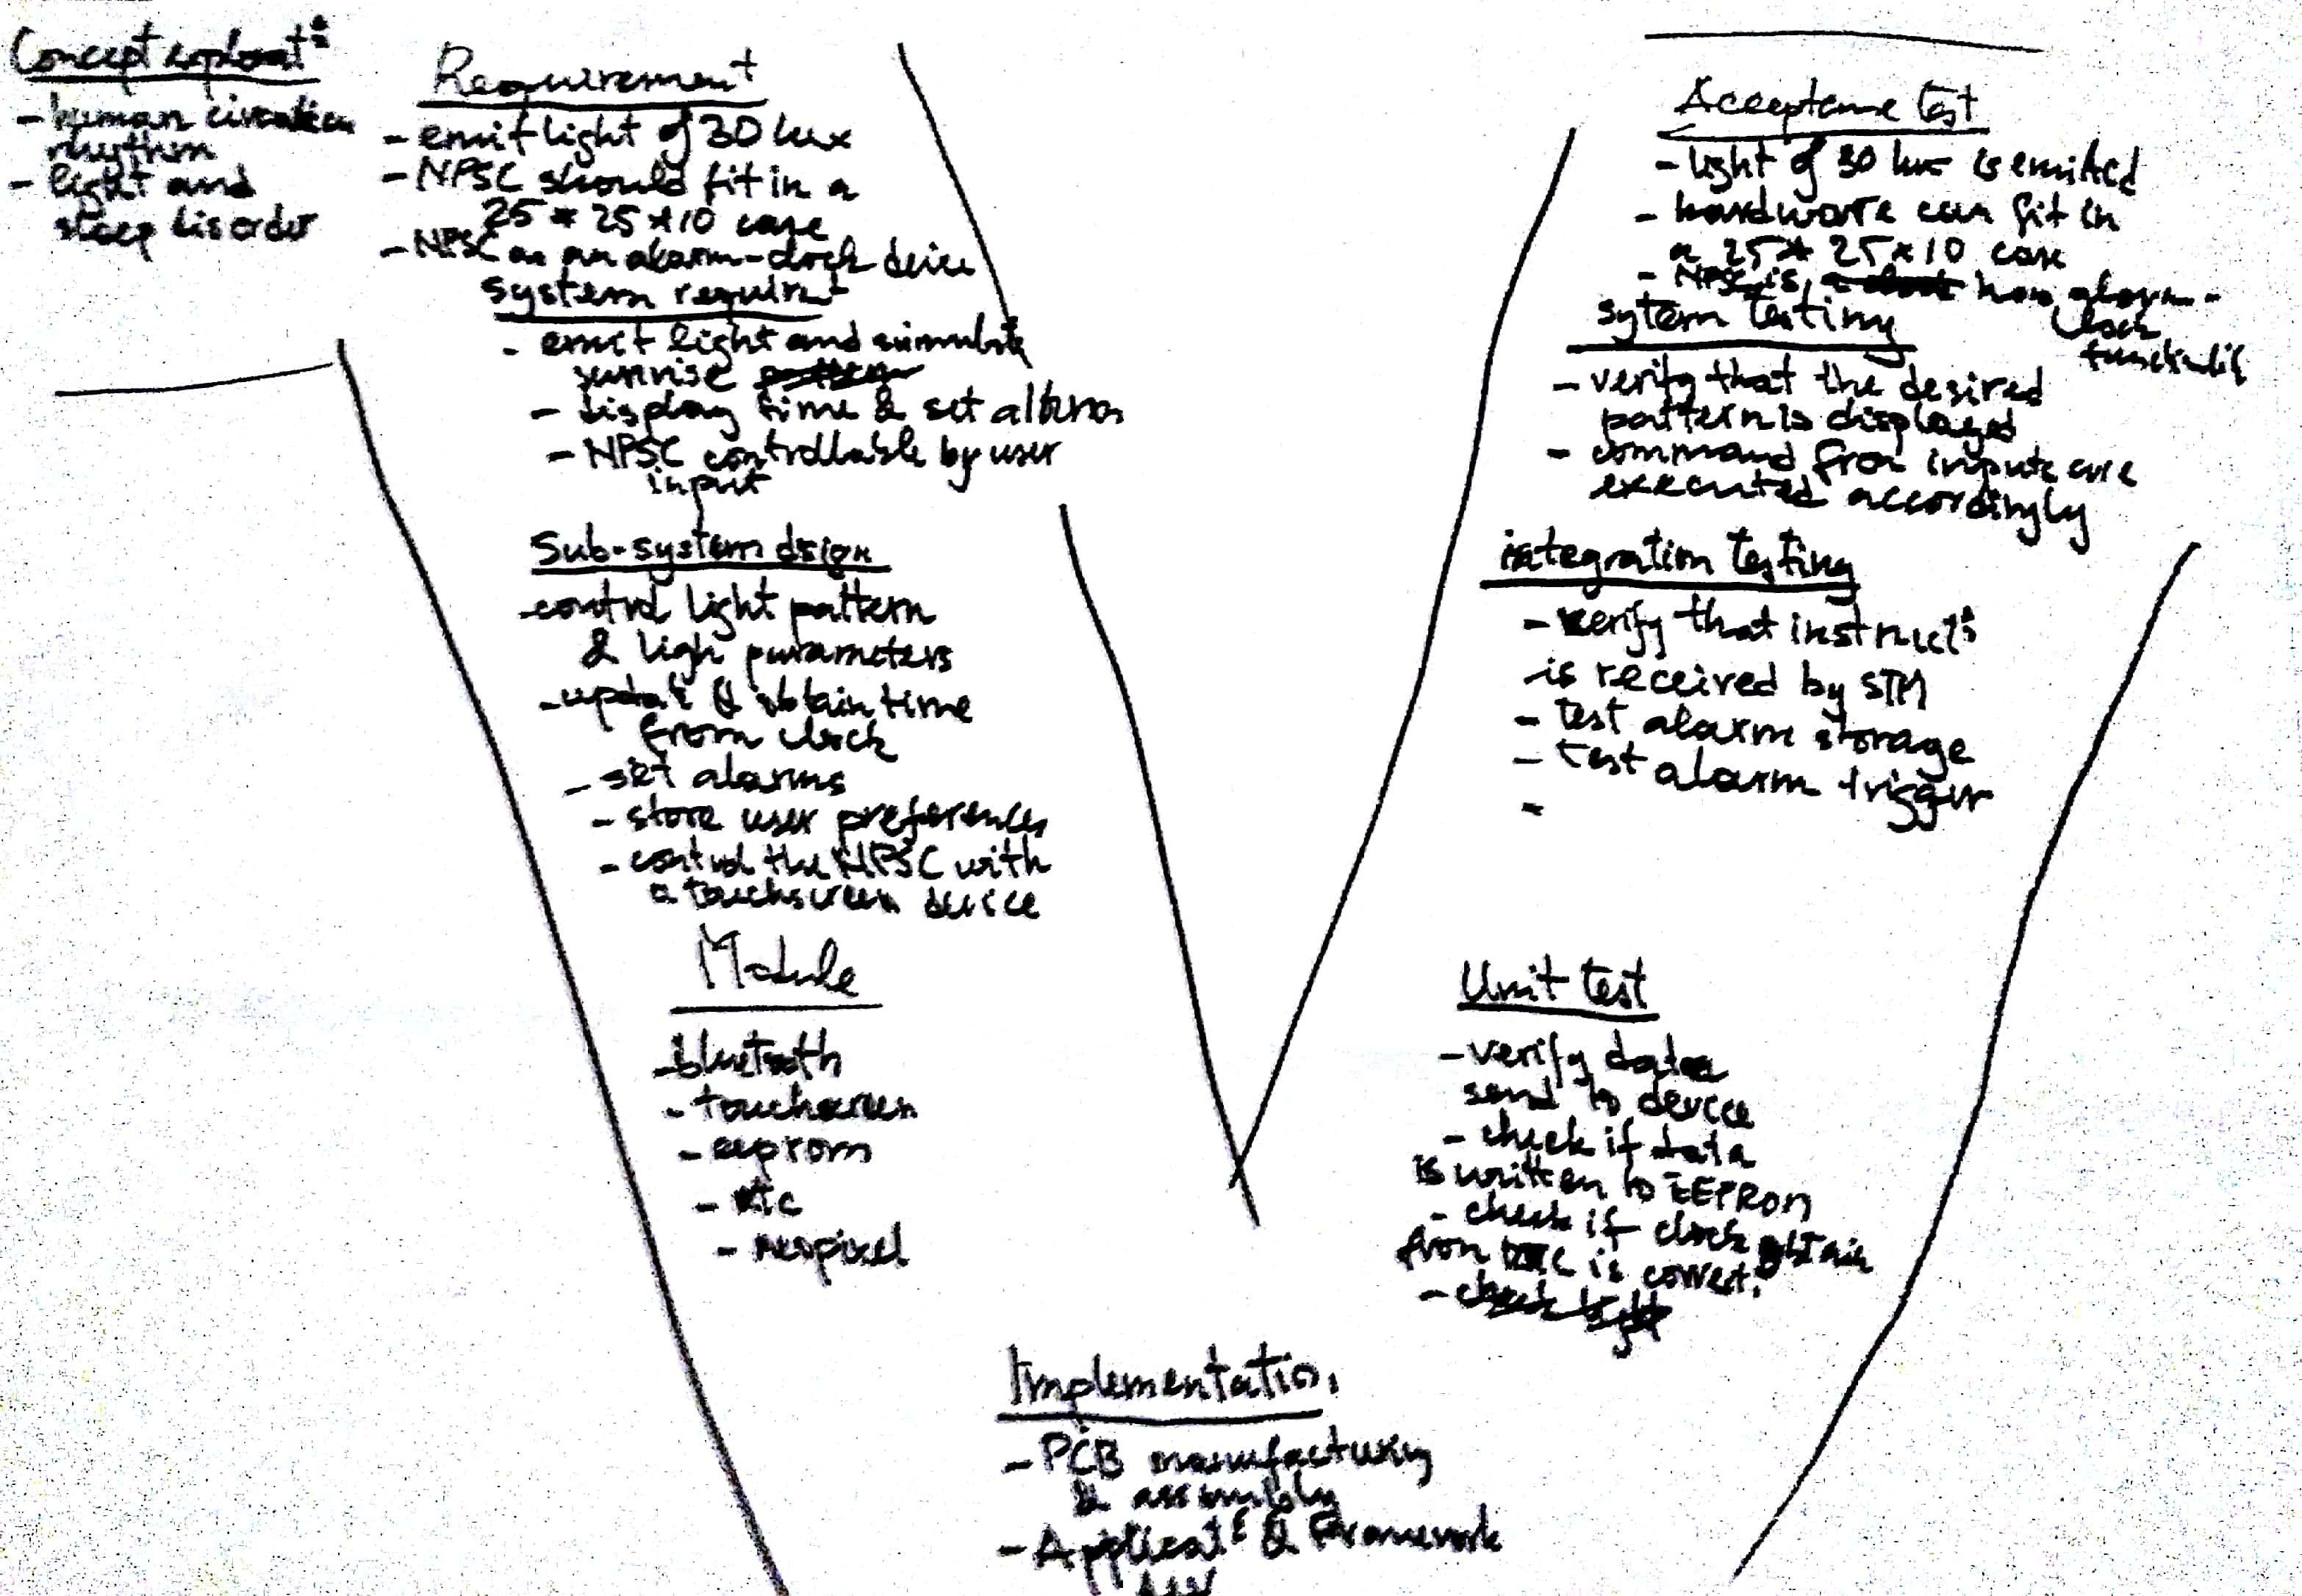
\includegraphics[scale=0.17]{v_diagram.jpg}
		\caption{V-diagram of the project. On the left side, from top to bottom are the verifications steps starting from the system requirements down to the modules. At the bottom is the implementation of the system On the right side, from the bottom to the top are the validations steps starting from the unit tests to the acceptance tests performed on the NPSC.}
		\label{fig:v_diagram}
	\end{figure}
\end{landscape}
%%%%%%%%%%%%%%%%%%%%%%%%%%%%%%%%%%%%%%%%%%%%%%%%%%%%%%%%%%%%%%%%%%%%%%%%%%%%%%%%%%%%
% SECTION: Hardware module
%%%%%%%%%%%%%%%%%%%%%%%%%%%%%%%%%%%%%%%%%%%%%%%%%%%%%%%%%%%%%%%%%%%%%%%%%%%%%%%%%%%%
\section{Hardware module tests}
The tests performed on the hardware are the basic hardware tests mentioned in \ref{basic_hardware_test}.
To ensure that the hardware were sending and receiving the right information, the \textit{Salea logic analyser} was used to analyse the data transmitted between the STM and the hardware modules.\Cref{table:coms_test} describes the communication tests performed on each module.

\begin{table}[h!]
	\centering
	\caption{Commnication protocol tests performed on hardware modules.}
	\label{table:coms_test}
	\begin{tabular}{cp{5em}p{25em}}
		\hline
		\hline
		\toprule
		\textbf{Hardware} & \textbf{Protocol} & \textbf{Test description}\\
		\hline
		\hline
		\toprule
		DS1307 & I2C & rtc\_setMinutes(10). Send the value 10 at address 0x01 of the RTC.\\ 
		\midrule
		25LC640 & SPI & eeprom\_write(10,0x00). Send SPI data of write type to write the value 10 at address 0x00.\\ 
		\midrule
		HC-06 & UART & bluetooth\_send(10). Send UART data of write type to send the value 10.\\ 
		\midrule
		NX4024T032\_001 & UART & nextion\_send(10). Send UART data of write type to send the value 10.\\ 
		\midrule
		MAX7221 & SPI &  date\_write(10,0x00). Send SPI data of write type to write the value 10 at address 0x00.\\
		\midrule
		WS2812 & PWM &  neopixel\_setAllPixelRGB(255,0,0) neopixel\_setAllPixelRGB(0,255,0) neopixel\_setAllPixelRGB(0,0,255). Send PWM data to the neopixels.\\
		\hline
		\hline
	\end{tabular}
\end{table}



%%%%%%%%%%%%%%%%%%%%%%%%%%%%%%%%%%%%%%%%%%%%%%%%%%%%%%%%%%%%%%%%%%%%%%%%%%%%%%%%%%%%
% SECTION: UnitTests
%%%%%%%%%%%%%%%%%%%%%%%%%%%%%%%%%%%%%%%%%%%%%%%%%%%%%%%%%%%%%%%%%%%%%%%%%%%%%%%%%%%%
\section{Unit tests}

Software unit tests could not be run on all hardware modules. It would have been impractical to set software unit tests on the Bluetooth module and the touchscreen as an application need to be developed using those modules before fully interacting with them. The Utilities modules and the Framework of the hardware modules tested using unit testing are listed in \cref{table:unitTest} alongside their unit tests.

\begin{table}[h!]
	\centering
	\caption{Unit tests performed on the Framework.}
	\label{table:unitTest}
	\begin{tabular}{ccp{18em}}
		\hline
		\hline
		\toprule
		\textbf{Hardware} & \textbf{Unit test} & \textbf{Description}\\
		\bottomrule
		\toprule
		\multirow{6}{*}{internal RTC} & test\_clock\_date & Assert that the date saved is the same as the date loaded from the internal RTC\\
		& test\_clock\_time & Assert that the time saved is the same as the time loaded from the internal RTC\\ 
		& test\_clock\_alarm & Assert that the alarm saved is the same as the alarm loaded from the internal RTC\\
		\midrule
		\multirow{3}{*}{external RTC} & test\_rtc\_clock & Assert that the clock written to the external RTC is the same as the one loaded from the external RTC\\
		\midrule
		\multirow{6}{*}{queue} & test\_queue\_create & Assert that a queue of specific datatype has been created\\
		& test\_queue\_enqueue & Assert that an element has been successfully added to the queue\\ 
		& test\_queue\_dequeue & Assert that an element has been removed from the queue\\
		\midrule
		\multirow{9}{*}{eeprom} & test\_eeprom\_write\_read & Assert that the byte written to the eeprom is the same as the byte read at the written address.\\
		& test\_eeprom\_write4B\_read4B & Assert that the a uint32\_t written to the eeprom is the same as the uint32\_t read at the written address.\\
		& test\_eeprom\_writeNB\_readNB & Assert that the N bytes written to the eeprom are the same as the N bytes read at the written address.\\
		\bottomrule
		\hline
		\hline
	\end{tabular}
\end{table}

%%%%%%%%%%%%%%%%%%%%%%%%%%%%%%%%%%%%%%%%%%%%%%%%%%%%%%%%%%%%%%%%%%%%%%%%%%%%%%%%%%%%
% SECTION: SystemTests
%%%%%%%%%%%%%%%%%%%%%%%%%%%%%%%%%%%%%%%%%%%%%%%%%%%%%%%%%%%%%%%%%%%%%%%%%%%%%%%%%%%%
\section{Integration tests}
The tests performed on the applications are more complex than the unit tests. It is important that the unit tests are run prior this tests as the applications rely on the framework. The description of all integration tests performed on the applications is shown in \cref{table:integrationTest}. 

\begin{table}[h!]
	\centering
	\caption{Integration test performed at the application level.}
	\label{table:integrationTest}
	\begin{tabular}{ccp{18em}}
		\hline
		\toprule
		\textbf{Application} & \textbf{Integration test} & \textbf{Description}\\
		\bottomrule
		\toprule
		\multirow{6}{*}{alarm} & test\_alarm\_address & Assert that the address of all type of the Alarm structure are offset by the correct memory size.\\
		& test\_alarm\_save\_load & Assert that the alarm save in the EEPROM is the one loaded from the EEPROM\\ 
		\bottomrule
		\hline
	\end{tabular}
\end{table}

%%%%%%%%%%%%%%%%%%%%%%%%%%%%%%%%%%%%%%%%%%%%%%%%%%%%%%%%%%%%%%%%%%%%%%%%%%%%%%%%%%%%
% SECTION: Ring
%%%%%%%%%%%%%%%%%%%%%%%%%%%%%%%%%%%%%%%%%%%%%%%%%%%%%%%%%%%%%%%%%%%%%%%%%%%%%%%%%%%%
\section{Neopixel Ring}
The Ring was designed so that it emits light with a wavelength of $460\pm 10nm$ and at an illuminance of  $30lux$ while being able to draw a current of $12A$ with a temperature rise of $15^oC$. Three experiments were conducted on the board to quantify its current consumption, its temperature rise and its illuminance.  

\subsection{Current experiment}
This experiment was done to verify that the board can draw $12A$ without blowing up (not kidding) and to find a mathematical model between the neopixel brightness and the board current consumption.\\
The first part of the consisted of finding the current drawn by a single neopixel based on its colour and brightness. The brightness levels are from 0\% to 100\% in steps of 10\%, so there were 11 brightness levels in total. The 0\% brightness level is defined as the idle state of the neopixel as all pixels are not turned on.\\
The second part of this test consisted of measuring the current consumption of the Ring with all 180 neopixels. Firstly the idle current of the board was measure (current when the board is powered and no data is sent). Secondly, the current per brightness level was measured.\\
In this experiment and all described below, the \textit{TOPWARD, DC power supply 33010D} capable of supplying a current of $10A$ was used.
\begin{figure}[ht]
	\centering
	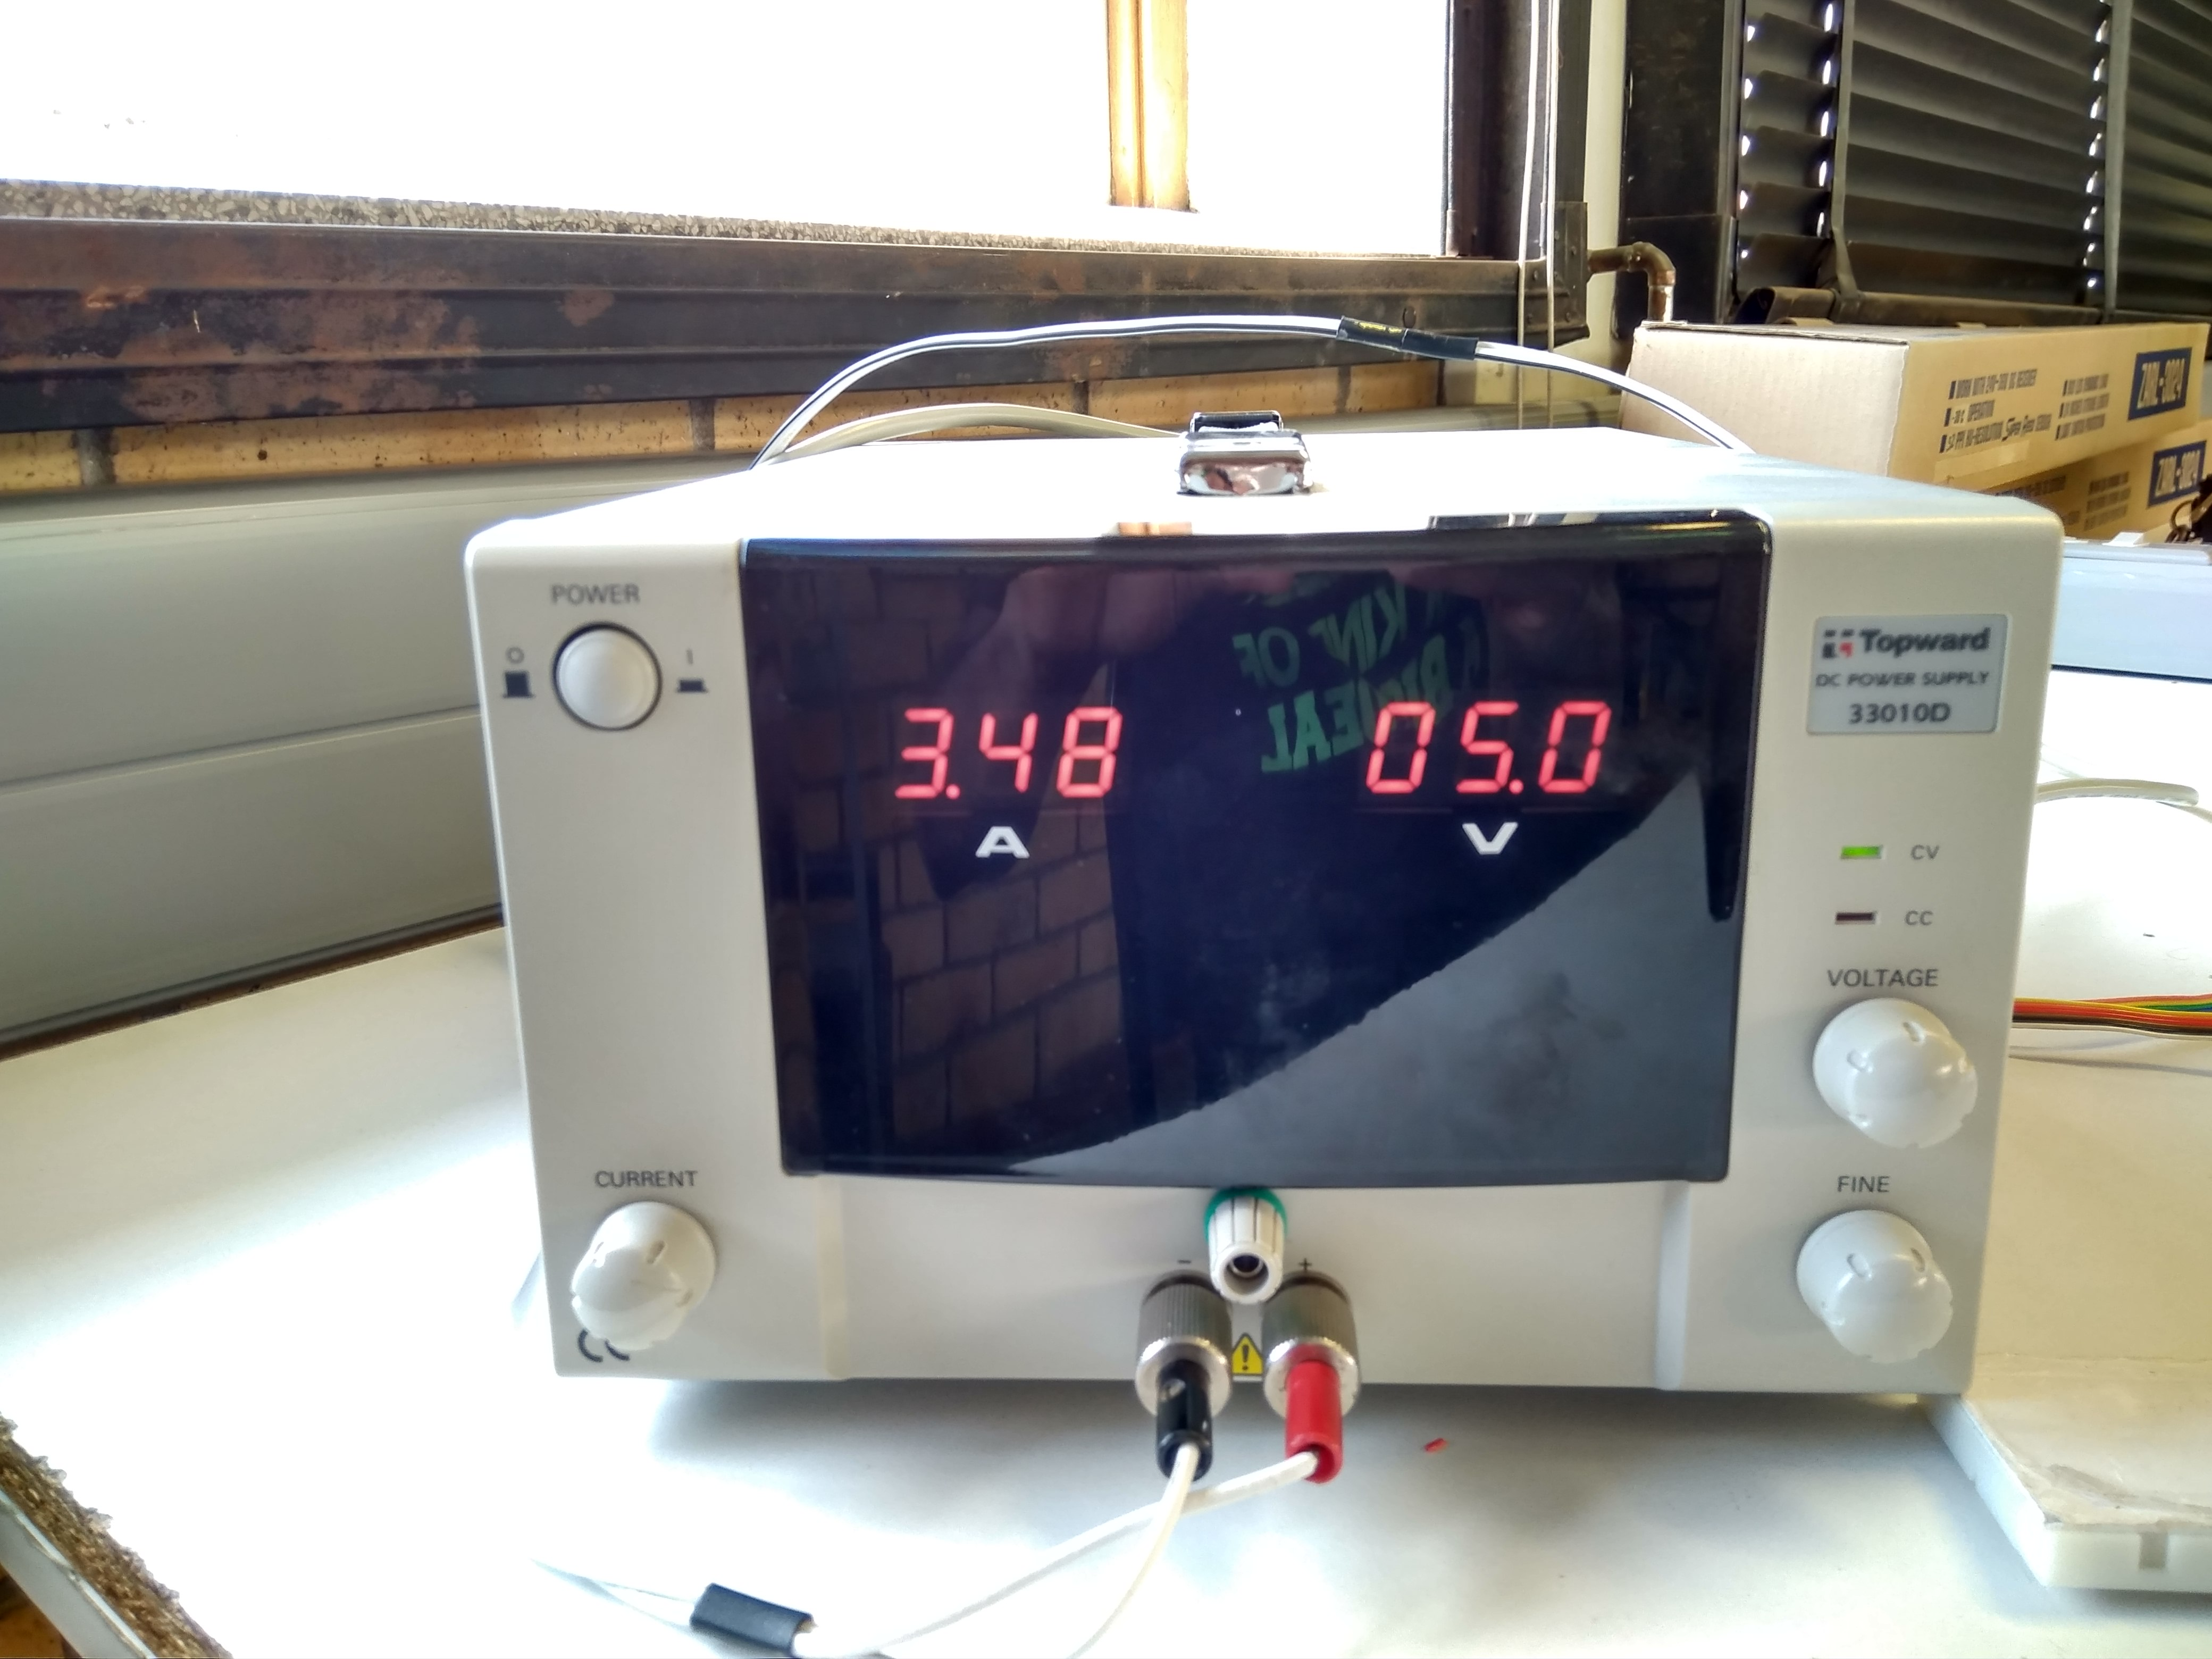
\includegraphics[scale=0.08]{power_supply.jpg}
	\caption{Power supply used in the Ring experiments.}
	\label{fig:power_supply}
\end{figure}
\subsection{Temperature experiment}
The temperature experiment was performed in order to find the temperature rise of the board per brightness level. In this experiment, all 180 neopixels were turned white (100\% red, 100\% green,100\% blue). \\
Four temperature sensors (MCP9700) were evenly placed at the back of the board as illsutrated by \cref{fig:test_temp_ring} to measure the board temperatue. Another temperature sensor was placed further away from the Ring to measure the room temperature. 
\begin{figure}[ht]
	\centering
	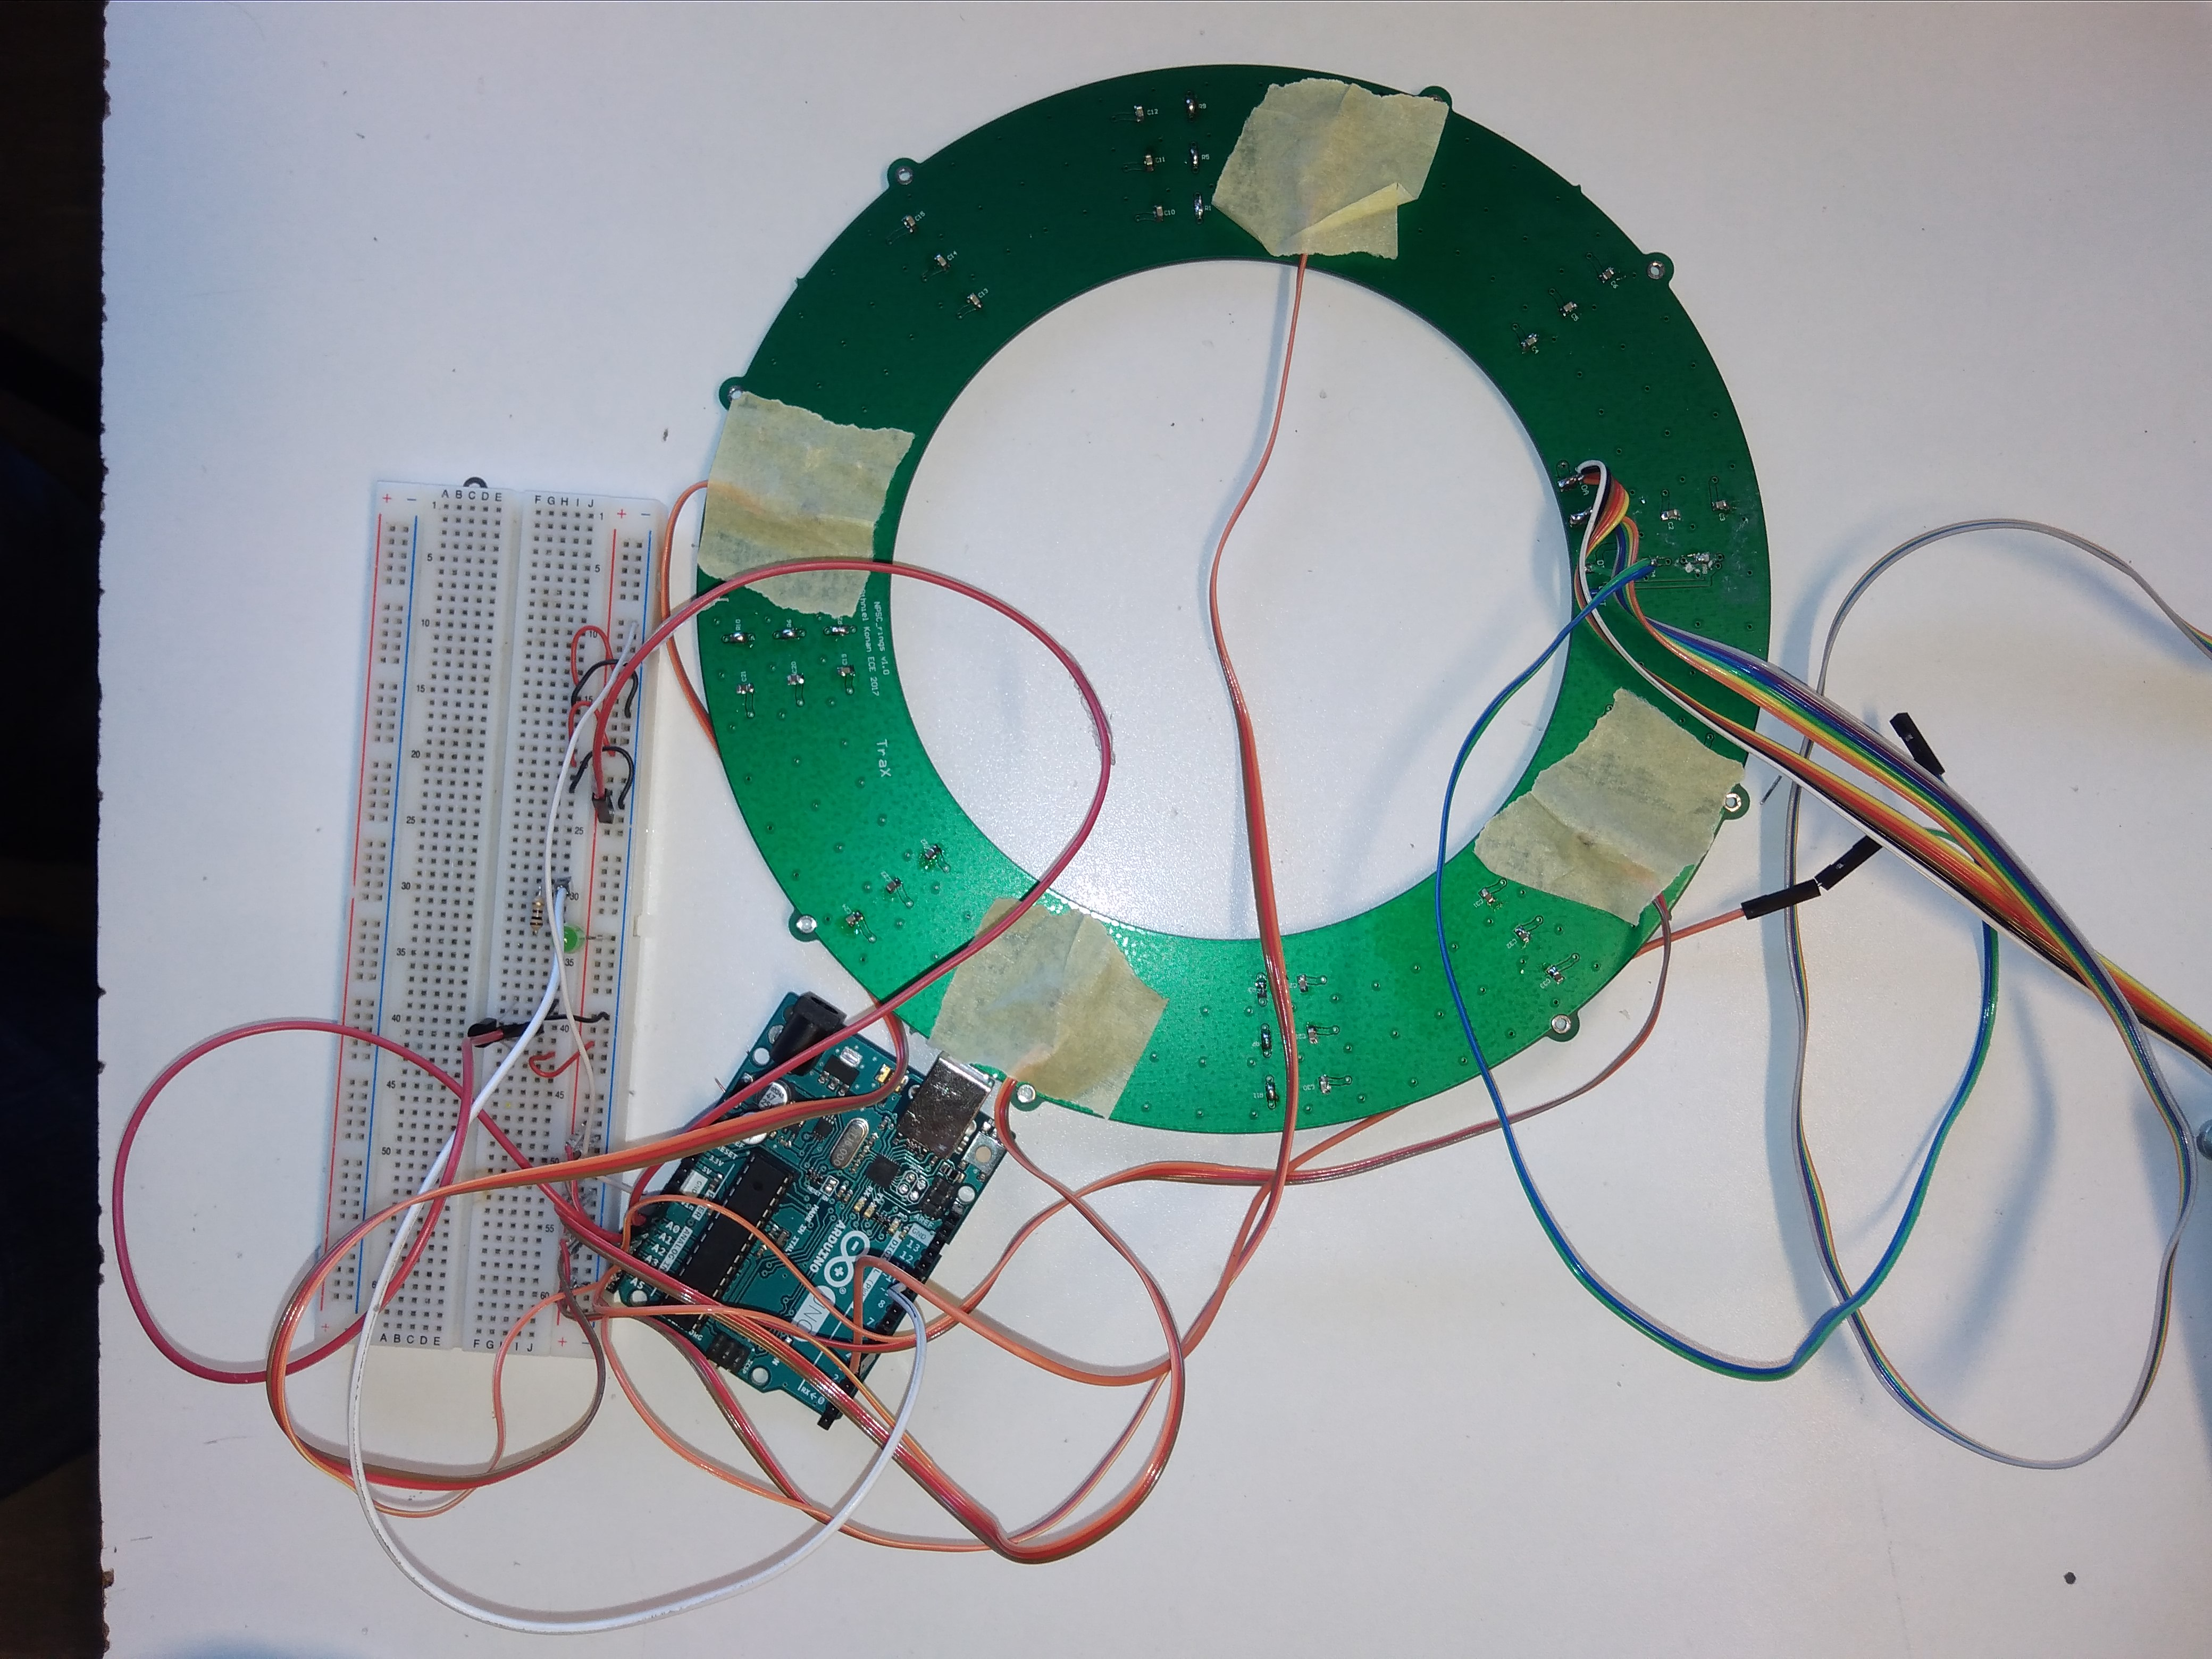
\includegraphics[scale=0.08]{test_temp_ring.jpg}
	\caption{Schematics used to obtain the board temperature.}
	\label{fig:test_temp_ring}
\end{figure}
An Arduino Uno was used to run this experiment by controlling the neopixels brightness and colour and by controlling the temperature sensors. The schematic in \cref{fig:temp_ring} was used to set up the experiment. In this schematic, $T_0$ is the temperature sensor measuring the room temperature and the temperature sensors $T_1$, $T_2$, $T_3$, and $T_4$ are the sensors placed on the board. Different power supplies were used in this experiment, the $5V$ @ $10A$ power supply was used to power the Ring while a $5V$ @ $0.5A$ power supply coming from the usb port of a laptop was used to power the Arduino and the temperature sensor. An LED was used to display the outcome of the experiment.
\begin{figure}[h!]
	\centering
	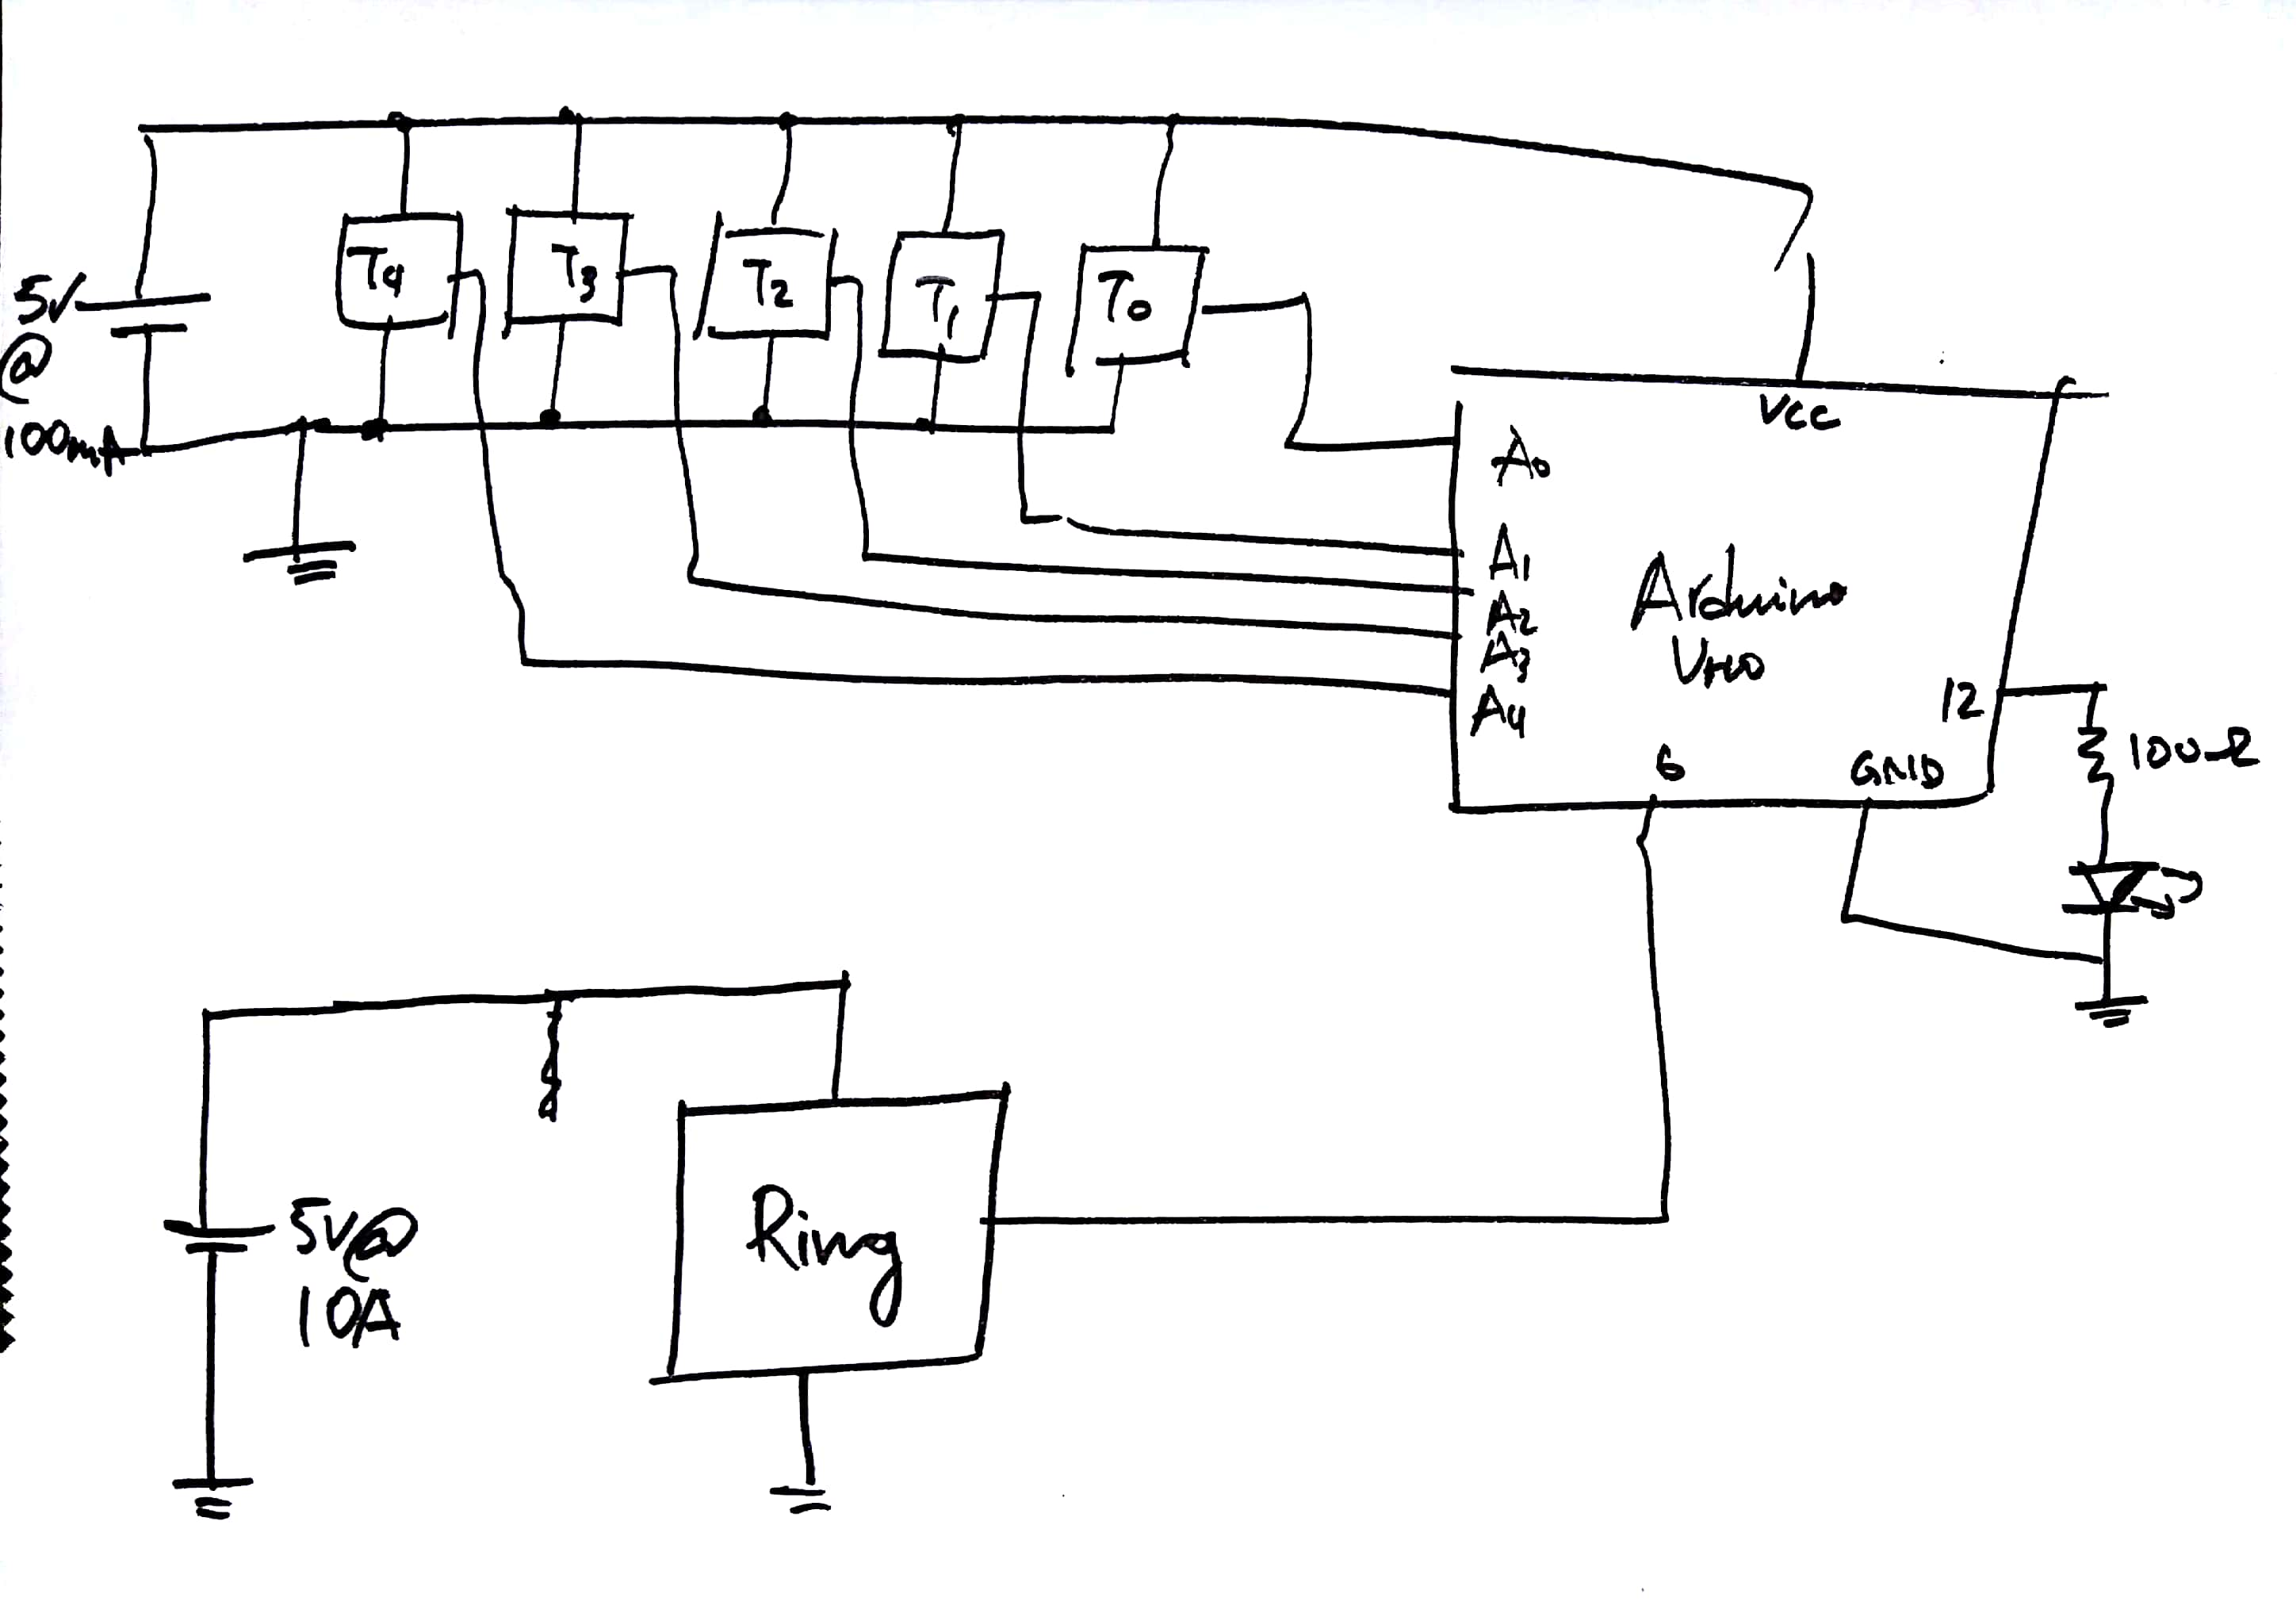
\includegraphics[scale=0.13]{temp_ring.jpg}
	\caption{Schematics used to obtain the board temperature.}
	\label{fig:temp_ring}
\end{figure}
Two programs were written for this experiment. The first program compares the average temperature given by sensors on the board with the room temperature and turns on the LED if those temperatures are the same. The second program averages the temperature of the sensors on the boards and display the sample number, the board temperature and the room temperature at interval of $10s$ on the Arduino's serial monitor.\\
The temperature of the board measure for each brightness level using all 180 neopixels with white colour. After each temperature measurement, the sensors were let to cool down to the room temperature using the first program written. The results of the experiment were taken from the serial monitor.\\
The overall setup of this experiment is shown in \ref{fig:temp_setup}.
\begin{figure}[h!]
	\centering
	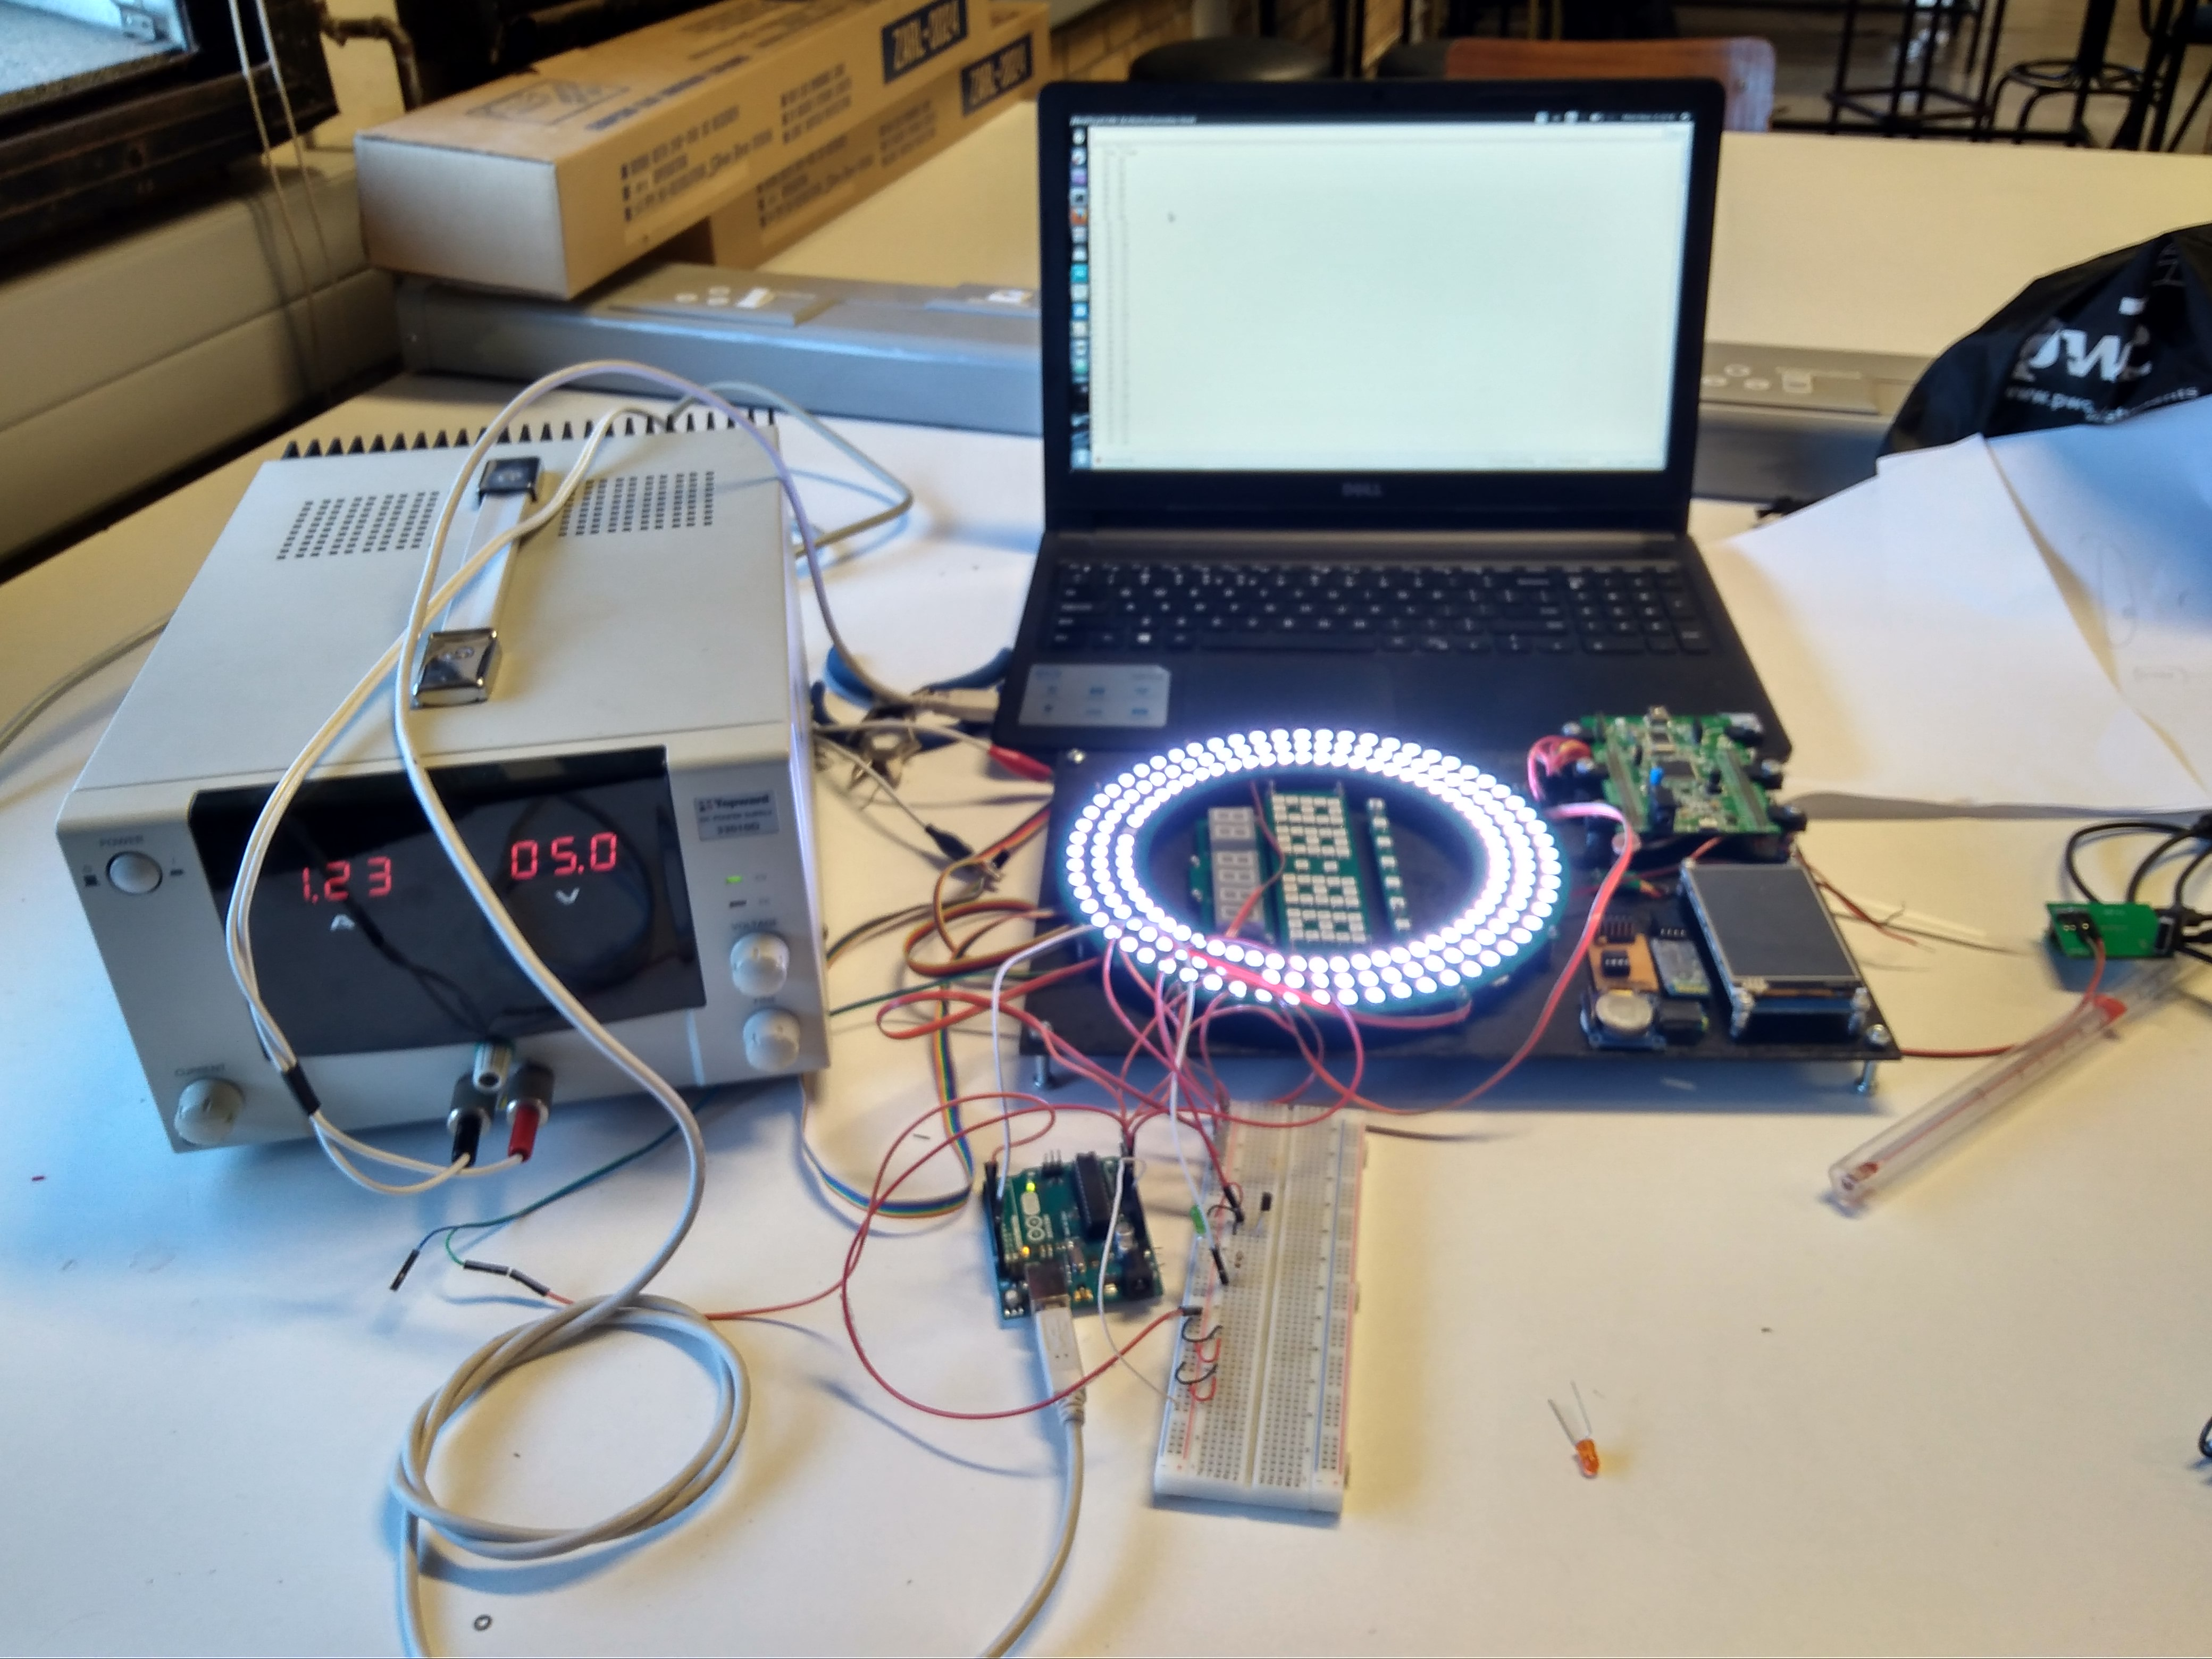
\includegraphics[scale=0.09]{temp_setup.jpg}
	\caption{Setup of the temperature rise experiment.}
	\label{fig:temp_setup}
\end{figure}

\subsection{Illuminance experiment}
This experiment was performed to quantify the illuminance of the Ring in order to verify if it meets its requirements. Moreover, the experiment's purpose was also to find a relationship between the distance and illuminance, the relationship between the angular position of the subject and the illuminance.\\
To ensure that the Ring's illuminance is properly measured, the experiment was performed in room EM6 in the Menzie Building at the University of Cape Town. The room's lights were turned off and all windows were closed so that a reading of $0 lx$ was obtained on the lux meter. The lux meter used in the experiment is the \textit{LTR55X ALSPRX}. It has a resolution of $0.01499930 lx$ and a maximum range of $10000.0 lx$. This lux meter is found in the \textit{Xiami Redmi 4} smartphone, it was used over other digital lux meters as there were not any available. For this reasons, the wavelength emitted by each LED of the neopixel could no be verified; only the lux emitted by the neopixel could be quantified.\\
The illuminance was measured for distances from the Ring ranging from $10cm$ to $100cm$ with steps of $10cm$. The experiment was performed at $0^o$, $30^o$, $60^o$, and $90^o$ angle, with the angle being measured from the normal to the front of the Ring. The Ring was placed on a table and the lines indicating the angles and the distance to the Ring was drawn on the same type of tables. \Cref{fig:test_illuminance} shows the positions of the Ring for the experiments. 
\begin{figure}[h!]
	\centering
	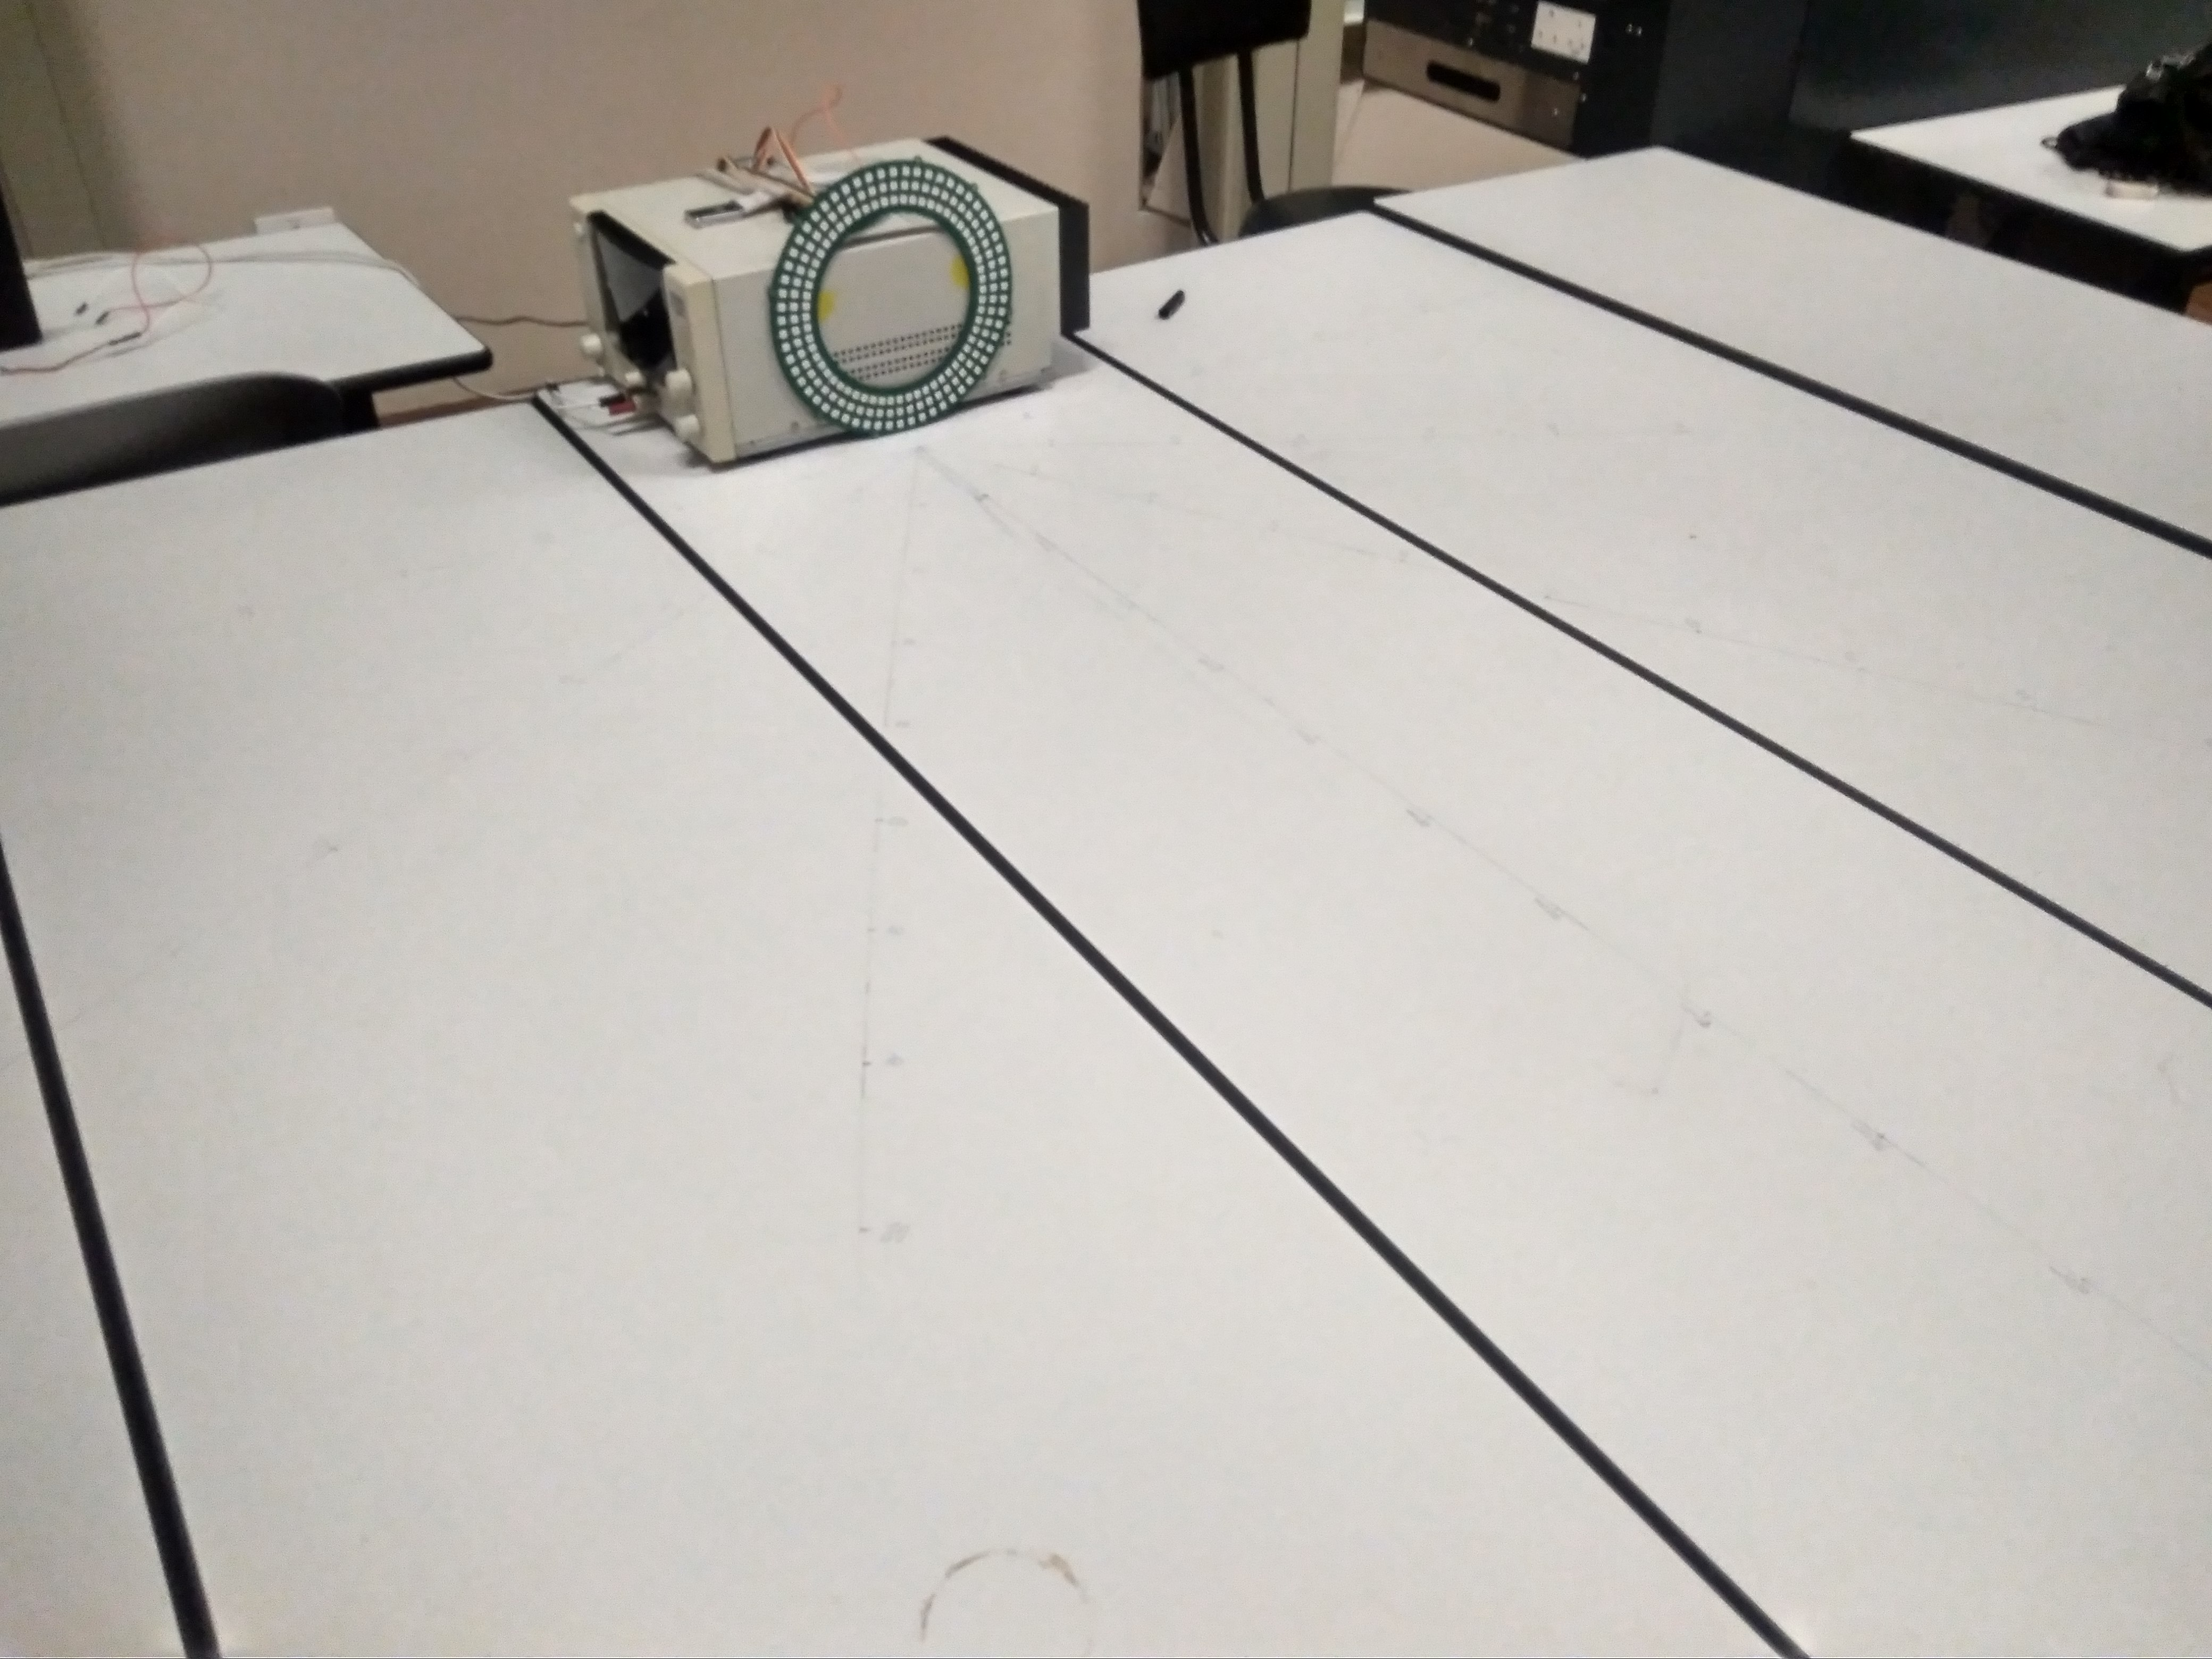
\includegraphics[scale=0.09]{test_illuminance.jpg}
	\caption{Illuminance test setup.}
	\label{fig:test_illuminance}
\end{figure}
After setting up the environment for the experiment, the illuminance of the Ring was taken at brightness level of $10\%$, $30\%$, $50\%$,$80\%$, and $100\%$. For each brightness the illuminance was measure at $0^o$, $30^o$, $60^o$, and $90^o$ angle. And for each angle, the brightness was measure at distance of $10cm$ to $100cm$ with steps of $10cm$.
